\documentclass[9pt, twocolumn, article]{memoir}
    \usepackage[utf8]{inputenc}
    \usepackage[T1]{fontenc}
    \usepackage[brazil]{babel}
    \usepackage[margin = 1.5cm]{geometry}
    \usepackage{times}
    \usepackage{graphicx}

\setlength{\parindent}{0cm}

\begin{document}

\section*{Introdução à IHC}

\textbf{1. Defina interface e interação.}\\
\textbf{Interface} é o ponto de interação entre diferentes sistemas e outras entidades (p.ex., usuário); é a parte visível pela qual o usuário mantém contato físico, têm acesso às funções e se comunica com o sistema interativo. Interação é o processo de comunicação entre usuários e computadores, ou quaisquer produtos, envolvendo tudo o que acontece quando o usuário, por meio da interface, interage com o sistema computacional para realizar tarefas. Na interação, o usuário e sistema trocam turnos em que um “fala” e o outro “ouve”, interpreta e realiza uma ação. Esta ação pode ser tão simples quanto dar uma resposta imediata à fala do outro, ou consistir de operações complexas que alteram o estado do mundo. 

Interface = Tudo aquilo com que o usuário entra em contato para interagir com o sistema, isso inclui hardware e software

\textbf{Fatores que influenciam na interação do usuário: } Percepção, memória, raciocínio. \textbf{Raciocínio: } \textbf{Dedução: } A partir de uma regra e uma observação,o usuário chega a uma conclusão.\textbf{Indução: } A partir de N observações, o usuário chega a uma conclusão.\textbf{ Abdução: } Como normalmente pensamos. A partir de uma observação, o usuário gera uma hipótese que ele considera verdadeira até que algo demonstre o contrário. Ao interagir com um sistema, o usuário.\\

\textbf{2. Por que a área de IHC é relevante para a Computação?}\\
Porque a computação gera sistemas com os quais o usuário precisa interagir. Nesse contexto, a IHC provê métodos e teorias que possibilitam a melhor interação e, consequentemente, melhor experiência para o usuário.

\textbf{3. Explique por que  IHC  é  considerada  uma  área  multidisciplinar  e  por  que  é  relevante  ter conhecimentos relacionados a:}\\
Um sistema computacional passa por muitos aspectos, não limitados apenas à computação. Dentre eles,
\textbf{a. Computação)} Precisa compreender possibilidades, limitações e adequação do sistema aos usuários;
\textbf{b. Psicologia)} As pessoas criam modelos mentais para interagir com o mundo e é preciso compreendê-los para criar um sistema compatível com a sua realidade;
\textbf{c. Ergonomia)} É preciso compreender as limitações e preferências físicas dos usuários para que o sistema potencialize as capacidades físicas durante a interação;
\textbf{d. Design)} Deve ser pensada além da estética, considerando a qualidade da interação e respeitando as condições dos usuários;
\textbf{e. Etnografia)} A interface pode gerar diferentes impactos sócio-culturais que devem ser compreendidos;
\textbf{f. Semiótica)} É preciso que as ideias criadas pelos usuários ao ver e interagir com o sistema sejam convergentes com o que ele quer representar;

\textbf{4. Descreva de forma resumida os seguintes estilos de interação:}\\
\textbf{a. Linguagem natural)} Linguagem sem domínio específico e sintaxe formal. Compreensão ``livre''.
\textbf{b. Linguagem de comando)} Linguagem bem estruturada e de domínio específico. Interpretação única.
\textbf{c. Menus)} Elementos agrupados por semelhança lógica; distintos e rotulados.
\textbf{d. Formulários)} Preenchimento de campos, agrupados logicamente.
\textbf{e. WIMP - Windows, Icons, Menus e Pointers)} Visualização de objetos interativos.
\textbf{f. WWW)} Uso de \emph{links} entre recursos.
\textbf{g. Realidade virtual)} Usuário ``faz parte'' do sistema.
\textbf{h. Interfaces tangíveis)} Interação com o software a partir de objetos tangíveis.
\textbf{i. Interfaces de ambiente)} Comunicação de informações através de recursos do ambiente.
\textbf{j. Interfaces Háptica)} Interação através de tato e força.

\textbf{5. Explique  o  que  são  qualidades  de  uso  e  qual  sua importância  no  contexto  de  interface  e interação}\\
Qualidades de uso são propriedades que qualificam a interação de acordo com determinados aspectos. São importantes porque uma interface de qualidade pode aumentar a produtividade e melhorar processos de negócio. Uma interface de qualidade permite a realização de tarefas de maneira eficaz, eficiente e agradável, ou seja, fornece uma melhor interação entre usuário e sistema.

\textbf{6. Explique     as    seguintes    propriedades:    Usabilidade,    Acessibilidade,    Comunicabilidade, Sociabilidade e Aplicabilidade.}\\
Usabilidade é a adequação do software às condições de uso. Acessibilidade é a capacidade do produto de atender ao maior número possível de usuários com ou sem necessidades especiais. Comunicabilidade é transmitir ao usuário as intenções e princípios de interação que a interface quer mostrar. Sociabilidade é a presença de políticas sociais compreensíveis, aceitáveis, implementáveis, que apoiam a proposta do grupo. Aplicabilidade é o sistema poder ser usado com sucesso em uma grande variedade de contextos, inclusive naqueles em que o objetivo do usuário diverge do pretendido.\\

\textbf{Acessibilidade na Web – 04 Princípios: } \textbf{Princípio 1: Perceptível: } A informação e os componentes da interface do usuário têm de ser apresentados aos usuários em formas que eles possam perceber .Ex:. Fornecer alternativa textual para conteúdo “não textual”.\textbf{ Princípio 2: Operável:} Os componentes de interface de usuário e a navegação têm de ser operáveis. Ex:. Conseguir navegar utilizando apenas o teclado. \textbf{Princípio 3: Compreensível: } A informação e a operação da interface de usuário têm de ser compreensíveis. Ex:. Ajudar os usuários a evitar e corrigir erros. \textbf{Princípio 4: Robusto: } O conteúdo tem de ser robusto o suficiente para poder ser interpretado de forma concisa por diversos agentes do usuário, incluindo tecnologias assistivas.


\textbf{7.É possível contemplar todos os atributos de usabilidade (em um mesmo sistema, sempre)?}
Nem sempre se consegue contemplar todos estes atributos em uma interface de usuário, apesar de ser desejável. Dependendo do contexto de utilização do produto, um ou outro atributo pode se tornar prioritário. Exemplo: caixa de um banco onde pode ter filas
e o tempo de atendimento é um aspecto crítico, os atributos “produtividade” e “prevenção de erros” tornam-se importantes.

\textbf{8. Diferencie Usabilidade e Comunicabilidade?}\\
Usabilidade diz respeito ao uso do sistema, enquanto comunicabilidade é a propriedade de transmitir ao usuário, de forma eficaz e eficiente, as intenções e princípios de interação que
guiaram o seu design. Tendo como premissa: a interface é uma comunicação do designer para o usuário. \\
\textbf{Alta Comunicabilidade: } O sistema comunica bem o que ele faz e o que ele não faz.\\ 
\textbf{Alta usabilidade: } O sistema está adequado ao uso de seu usuário de forma que ele seja considerado produtivo e fácil de usar.\\

\textbf{Alta Comunicabilidade e Baixa Usabilidade?} É possível. O sistema pode comunicar bem as intenções de projeto da sua interface (para que ele serve, para quem e o que pode ser feito). Porém, ele
pode não atender as necessidades/objetivos do usuário ou ainda, não ser produtivo.\\
\textbf{Baixa Comunicabilidade e Alta Usabilidade?} Não é possível. Se o sistema não transmite de forma adequada como deve ser utilizado, o usuário terá problema durante a interação dificultando o uso e a produtividade.

\section*{Teorias da IHC}

\textbf{1. Segundo  a  teoria  das  ações  o  usuário  deve  transpor  os  golfos  de  execução  e  avaliação  para conseguir interagir com o sistema. Descreva as etapas que devem ser executadas para transpor cada um dos golfos}\\
Golfo de execução: formular intenções, especificar sequência de ações, executar. Golfo de avaliação: perceber estado do sistema, interpretá-lo, avaliar em relação à interação. Basicamente, o usuário olha para a interface, formula sua intenção, especifica a sequência de ações e executa. A partir de sua percepção da resposta, ele a interpreta e avalia os resultados.

\textbf{2. Um usuário está logado no Facebook e deseja deixar um recado de Feliz Aniversário para o seu amigo aniversariante do dia.  Baseado na teoria das ações da Engenharia Cognitiva, como esse usuário  vai  agir,  para  interagir  como  sistema?  Descreva  cada  etapa  dos golfos de execução e avaliação}\\
1. formular interação: ``quero mandar parabéns''; 2. especificar ações: ``tenho que ir à página dele e preencher o campo de recado''; 3. executar $\rightarrow$ recado postado; 4. perceber: ``a página mudou''; 5. interpretar: ``aqui está o meu recado''; 6. avaliar: ``deu certo''.

\textbf{3. Segundo   a   Engenharia   Cognitiva,   é   correto  afirmar  que a distância  articulatória  está relacionada ao golfo de execução, enquanto a distância semântica está relacionada ao golfo de avaliação? Justifique.}\\
Não, pois ambas distâncias existem nos dois golfos. Elas têm a ver com os significados e formas na interface, portanto envolvem ação e avaliação.

\textbf{4. Explique  o  que  é  a  Teoria  da  Engenharia  Semiótica  e os  principais  pontos  da  teoria, relacionados ao fenômeno de interação.}\\
Trata-se de uma teoria de design baseada em comunicação. Considera ambientes mono e multiusuários; compreende que um signo pode ter várias interpretações por diferentes usuários; e orienta a utilizar signos que geram semioses convergentes. Assim, a interação pode ser realizada de formas diferentes, mas atingindo, preferencialmente, o mesmo objetivo.

\textbf{5. Apresente a classificação da Engenharia Semiótica para signos.}\\
O conceito geral que se refere a todas as coisas que têm um significado (qualquer) para alguém é denominado signo. Para tal, há três classificações: Metalinguístico: elementos que auxiliam a compreensão do sistema. Estáticos: elementos que representam o estado do sistema -- desacoplamento temporal e causal. Dinâmicos: representam o comportamento do sistema -- acoplamento temporal e causal.

\textbf{6. Considere a interface e interação do Sistema Acadêmico do CEFET. A partir dessa interface, dê um exemplo de signo metalinguístico, estático e dinâmico.}\\
Metalinguístico: instruções na página de login. Estático: formulário de login. Dinâmico: ação de entrar no sistema ao clicar no botão ``entrar''. 

\textbf{9. Quais as principais diferenças entre a Teoria da Engenharia Cognitiva e a Teoria da Engenharia Semiótica?}\\
Semiótica: mono/multiusuário; múltiplas interpretações; múltiplas soluções; auxílio do projetista. Cognitiva: monousuário; interpretação única; objetivo bem definido; sem auxílio ao design.

\textbf{10.\\Formulação da Intenção: trocar todas as ocorrências de /Elisa/ por /Eliza/, observando maiúsculas e minúsculas} \\Golfo de:

Especificação da Sequencia de Ações/ (Execução das Ações):
I. Ação: Ativar ferramenta de localização e substituição\\a. Execução das Ações:\\
II. Ação:\\
a. Execução das Ações:\\
Digitar ‘Elisa’ no campo correspondente a ‘Localizar’ e\\
b. Execução das Ações:\\
Digitar ‘Eliza’ no campo correspondente a ‘Substituir por’\\
III. Ação: Assinalar que a operação deve preservar maiúsculas e minúsculas\\
a. Execução das Ações:\\
IV. Ação:\\
b. Execução das Ações:\\
Clicar no botão rotulado ‘Substituir tudo’\\
Golfo de: \\
Etapa de Percepção: O usuário percebe uma rápida ‘piscada’ do monitor e vê a janela de diálogo no seguinte
estado:\\
Etapa de:\\
Etapa de:\\

\textbf{12. Explique e diferencie os diferentes tipos de  Processos de Design (Centrado no Usuário; Estrela; Eng. Usabilidade de Nielsen e Design como Comunicação)}
\emph{Design centrado no usuário} foca na presença do cliente no início e durante a avaliação do ciclo: 1. identificação de requisitos $\leftrightarrow$ 2. (re)design $\leftrightarrow$ 3. construção de versão interativa $\leftrightarrow$ 4. avaliação (daqui, pode-se voltar 1 ou 2); o processo é iterativo. \emph{Modelo em estrela} tem cinco faces: análise de usuários/tarefas/funcional, especificação de requisitos, design, prototipação e implementação; antes de mudar de etapa, deve-se sempre fazer uma avaliação. Além disso, pode-se começar por qualquer uma das cinco fases, tornando-o muito flexível e dificultando o gerenciamento dos processos. \emph{Engenharia de usabilidade} é um processo sequencial em que as características de usabilidade são definidas antes, de forma quantitativa, e medidas durante o processo. Se parece com processos de engenharia de software e pode ser escalado para pequenos projetos. \emph{Design como comunicação} também segue o ciclo de análise, projeto e avaliação, embora se baseie na engenharia semiótica para realizar o projeto como a elaboração de uma metamensagem. Faz uso dos signos e prioriza comunicabilidade para gerar usabilidade e acessibilidade.\\

\textbf{Sociabilidade - Diretrizes/Princípios:}\textbf{E1} - Permitir que as pessoas desenvolvam suas próprias identidades
online,
\textbf{E2 }- Encorajar a empatia e confiança entre os membros. 
\textbf{E3 }- Encorajar a reciprocidade, 
\textbf{E4 }- Manter discussões em evidência e em tópicos, 
\textbf{E5 }– Manter possibilidades diversificadas de comunicação e interação publicas e privadas, 
\textbf{E6 }- Garantir proteção e privacidade.\\

\textbf{Interface como Metacomunicação:} Para a Engenharia Semiótica, a interface de um sistema é entendida como uma comunicação, unidirecional e indireta, do projetista aos
seus usuários

\textbf{Signos Metalinguísticos:} se referem a outros signos da interface. Usado pelos designers para explicitamente comunicar aos usuários os significados codificados no sistema e como podem utilizá-los.
\textbf{Signos estáticos:} podem ser interpretados independente de relações causais ou temporais. O contexto de interpretação é limitado aos elementos presentes na interface em um dado momento. Expressam o estado do sistema.
\textbf{Signos Dinamicos:} representam o comportamento do sistema, ou seja, estão relacionados aos aspectos temporais e causais da interface. Só podem ser percebidos através da interação com o
sistema. \\
Os signos metalinguísticos nos fornece uma visão geral do sistema. Os signos estáticos ajudam a responder, com mais detalhes, as questões relacionadas ao que o usuário deseja fazer. Os signos dinâmicos ajudam a responder, com mais detalhes, a questão referente a ”como interagir” para alcançar o objetivo.

\textbf{Signo:} Qualquer coisa que represente algo para alguém. Composto simultaneamente por: Objeto, Representamen (sua representação) e Interpretante (o que ele significa).
\textbf{Sistema de Significação: } Codificação entre expressão e conteúdo – utilizar um elemento para expressar algo (e.g., a ação “Salvar” codificada no signo ).\textbf{ Processo de significação: } processo através do qual expressão e conteúdo de signos são
estabelecidos com base em convenções sociais e culturais conhecidas das pessoas que vão utilizá-los, produzindo e interpretando signos (i.e., significado atribuído a um signo de acordo com o contexto cultural e social)

\textbf{Design Centrado no Usuário: }
\textbf{1.} Foco no usuário no início do processo de design e avaliação do artefato.
\textbf{2.} Identificar, documentar e chegar a um acordo sobre
requisitos de qualidade específicos (e.g. usabilidade, comunicabilidade, aprendizado, experiência do usuário)
\textbf{3.} Iteração é inevitável
a. Ninguém nunca acerta na primeira vez \\

\textbf{Ciclo de Desenvolvimento Estrela}
Pode começar por qualquer uma das etapas. A “Avaliação” fica no centro, pois a ideia é que a cada etapa a equipe possa avaliar a situação antes de passar para próxima etapa. Não é muito utilizado na prática (indústria). Talvez por ser flexível demais e
dificultar o gerenciamento das atividades, a não ser que se altere o
modelo. \\

\textbf{Engenharia de Usabilidade: }é um processo através do qual as
características de usabilidade são especificadas, antecipadamente e de forma quantitativa no processo de desenvolvimento, e medidas durante todo o processo. Fluxo gerencial e Fluxo técnico. 
Visão holística de engenharia de usabilidade. Fornece ligação a abordagens de engenharia de software. Ciclo de vida envolve: etapas de identificação de requisitos, design, avaliação e prototipação.Definição dos objetivos de usabilidade fazem parte da primeira etapa (análise de requisitos). Pode ser escalado para projetos pequenos. Utiliza um guia de estilo para registrar objetivos de usabilidade.

\textbf{Design Baseado em Cenários:} Utiliza diferentes tipos de cenários como representação básica e fundamental durante todas as
atividades envolvidas na concepção e uma solução de IHC. \textbf{Vantagens: } Normalmente escritos em linguagem natural, facilita o entendimento de todos os envolvidos e estimula a sua participação; Geração de cenários estimula a discussão e análise do impacto da tecnologia nos usuários e suas atividades; Encorajam a análise de caminhos alternativos (“e se…?”) e a imaginação da equipe de design.


\textbf{Design como Comunicação: } Entende que cada usuário forma
sua semiose diante dos signos, logo um mesmo signo pode ter múltiplas interpretações por usuários distintos. Inclui o projetista como elemento importante do processo. Orienta que os designer utilizem signos que possam desencadear semioses convergentes (similares) em torno de um significado dentro de um projeto de interface e interação.\\
\textbf{Design Centrado no Usuário: } Idealização de que todos os
usuários são iguais e de que só existe uma única possibilidade de
interpretar a interface de um sistema. Não inclui o “projetista de
interface” como elemento importante do processo.



\centering
\begin{figure*}
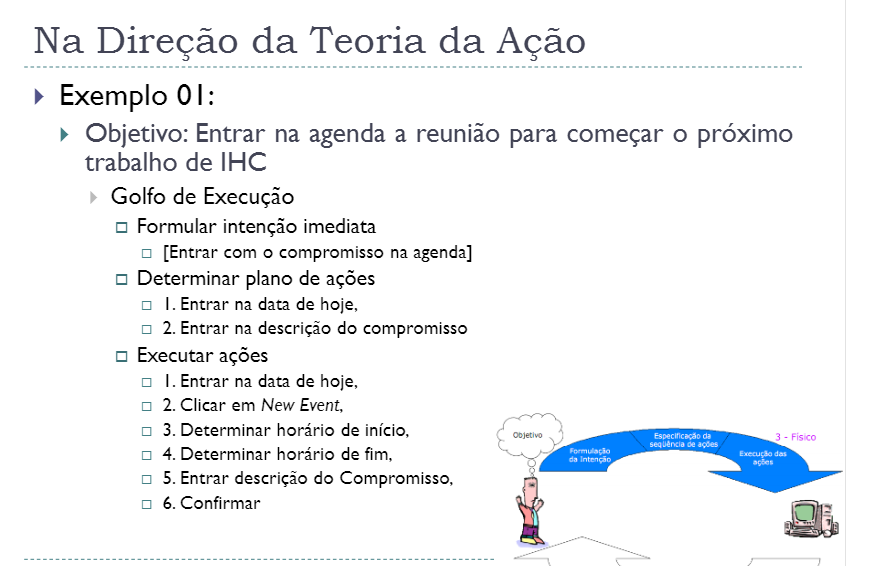
\includegraphics[width = 0.8\textwidth]{1.png}\\

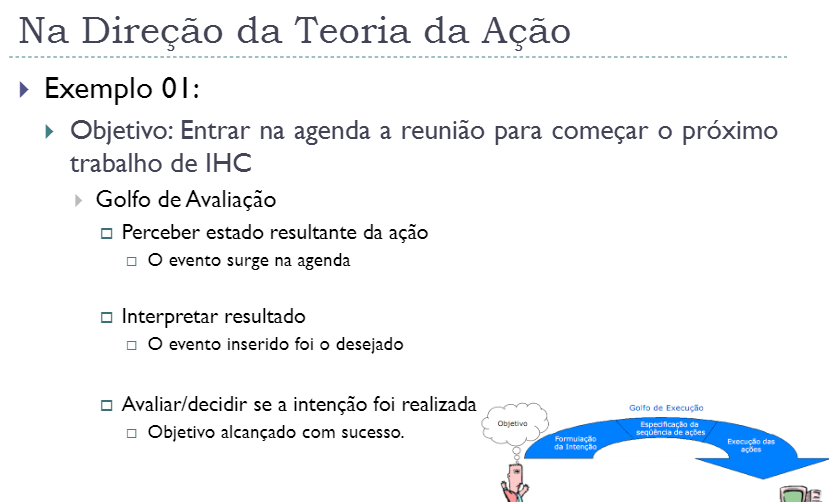
\includegraphics[width = 0.8\textwidth]{2.png}\\
\end{figure*}



\end{document}
